%--------------------------------------------------------------------------------------%--------------------------------------------------------------------------------------
%
%  Global settings, dont change it! (excapt additional \usepackage commands)
%  Always use PDFLatex!
%
%--------------------------------------------------------------------------------------%--------------------------------------------------------------------------------------
\documentclass[a4paper, 12pt, oneside, BCOR1cm,toc=chapterentrywithdots]{scrbook}

\usepackage{graphicx}           % use for pdfLatex
\usepackage{makeidx} % f\"{u}r Benutzung des Befehls \printindex
\usepackage[colorlinks=false]{hyperref}
\usepackage{tocbibind}
\usepackage{blindtext}
\usepackage{subfigure} 
\usepackage{acronym}
\usepackage{amsmath}
\usepackage{gensymb}
\hypersetup{%
bookmarksnumbered=true, hyperindex=true,
%
%Im Acrobat Reader Subtitel 1. Ebene anzeigen
bookmarksopen=true, bookmarksopenlevel=1,
%
pdfborder=0 0 0 % Keine Box um die Links!
}

% --------------------------------------------------------------
% Force Tables and List to be added in Table of Content
% --------------------------------------------------------------

\renewcommand*{\tableofcontents}{%
  	\begingroup
  	\tocsection
  	\tocfile{\contentsname}{toc}
  	\endgroup
}
\renewcommand*{\listoffigures}{%
  	\begingroup
  	\tocsection
  	\tocfile{\listfigurename}{lof}
  	\endgroup
}
\renewcommand{\listoftables}{
	\begingroup
	\tocsection
	\tocfile{\listtablename}{lot}
	\endgroup
}
\begin{document}

%--------------------------------------------------------------------------------------%--------------------------------------------------------------------------------------
%
%  Here starts the userspace !
%
%--------------------------------------------------------------------------------------%--------------------------------------------------------------------------------------

%--------titlepage
\begin{titlepage}

{
    \begin{center}
        \raisebox{-1ex}{
\includegraphics[scale=1.5]{TU_Chemnitz_positiv_gruen.pdf}}\\
    \end{center}
    \vspace{0.5cm}
}

\begin{center}

\LARGE{\textbf{Driver head orientation detection using Transfer Learning}}\\
\vspace{1cm}


\Large{\textbf{Research Project}}\\ 
\vspace{1cm}
Submitted in Fulfilment of the\\
Requirements for the Academic Degree\\
M.Sc.\\
\vspace{0.5cm}
Dept. of Computer Science\\
Chair of Computer Graphics and Visualization
\end{center}
\vspace{2cm}
Submitted by: Adarsh Mallandur\\
Student ID: 457084\\
Date: 19.09.2018\\
\vspace{0.3cm}\\
Supervising tutor: Stephen Helmert \\

\end{titlepage}

%---------------------------------------------------------
% Abstract
%---------------------------------------------------------

\addchap*{Abstract}
Estimating the head pose of the driver is a crucial as well as one of the difficult problems in the task of driver attention monitoring systems, given the problems of occlusions, illumination changes and the different poses of the driver. It is useful especially in highly autonomous vehicles where the handoff time to human driver needs to be determined. Traditionally head pose is estimated by detecting facial landmarks and solving the problem of 2D to 3D correspondence. This is a fragile method since it depends entirely on the estimation of landmarks which is difficult especially when there are occlusions and variations in illuminations. In this research project, a more robust way of estimating the head pose is done by training a convolutional neural network through the method of transfer learning. In our case, a network pre-trained on ImageNet dataset is used as feature extractor and further trained on DrivFace, a dataset containing images sequences of subjects while driving in real scenarios. This network classifies the RGB images into three classes: looking left, looking front and looking right. Results show that the method of transfer learning overcomes a DeepaGaze, a head pose estimation framework trained on in-the-wild datasets.
\\\\
\textbf{Keywords: Convolutional neural networks, transfer learning, head pose estimation, deep learning}

%---------------------------------------------------------
% Table of Contents, List of figures, List of Tables
%---------------------------------------------------------

\tableofcontents
\listoffigures
\listoftables

%---------------------------------------------------------
% List of Abbreviations
%---------------------------------------------------------
\twocolumn
\addchap{List of Abbreviations}
\begin{acronym}[Bash]
 \acro{ADAS}{Advanced Driver Assistance Systems}
 \acro{CNN}{Convolutional Neural Networks}
 \acro{IVIS}{In-Vehicle Information Systems}
 \acro{AFLW}{Annotated Facial Landmarks in the Wild}
 \acro{ReLU}{Rectified Linear Unit}
 \acro{ANN}{Artificial Neural Network}
 \acro{SGD}{Stochastic Gradient Descent}
 \acro{LSTM}{Long Short Term Memory}
\end{acronym}

\onecolumn
%---------------------------------------------------------
% Here starts the real work
%---------------------------------------------------------

\chapter{Introduction}
 Driver attention monitoring in real time is a crucial task of advanced driver assistance systems. The driver drowsiness and distraction from the road increases the risk of accident significantly \cite{noauthor_impact_nodate} \cite{liang_how_2012}. The use of in-vehicle information systems (IVISs) such as cell phones, GPS navigation systems, and satellite radios further adds to the risk. \cite{strayer_cell_2003} \cite{lee_speech-based_2001}Hence it is necessary to design driver attention montoring systems. One way this could be helpful is to capture the driver distractions and alert the driver in case of dangerous situations. There has been lot of work done in developing driver attention monitoring in the context of Advanced Driver Assistance Systems(ADAS) \cite{liang_real-time_2007} However, there is no system which generalises the driver head pose estimation across various drivers, cars and perspectives. Convolutional Neural Networks (CNNs) have been successful in various image classification and object detection tasks \cite{krizhevsky_imagenet_2017}. In this project, the feasibility of CNNs in driver monitoring systems is analysed. 
 
\section{Problem statement}
 
The aim of this project is to use CNNs to classify the driver gaze zones. However training CNNs from scratch is often time consuming and difficult. It requires learning of millions of parameters and a large number of annotated images for training. Training CNNs for smaller datasets often leads to overfitting. Transfer learning solves this problem by using pre trained weights learnt by CNNs on large scale datasets. \cite{noauthor_survey_nodate} In this project, two different networks trained on the ImageNet \cite{krizhevsky_imagenet_2012} dataset is fine tuned to classify driver gaze zones in the DrivFace dataset \cite{noauthor_uci_nodate}. The DrivFace database contains images sequences of subjects while driving in real scenarios. It is composed of 606 samples of 640*480 pixels each, acquired over different days from 4 drivers (2 women and 2 men) with several facial features like glasses and beard. The performance of the transfer learning network on DrivFace dataset is compared against Deepgaze \cite{noauthor_head_nodate} , a CNN trained on AFLW dataset \cite{noauthor_icg_nodate}.

\section{Structure of the project}
The main focus of this project work can be summarised as

\begin{enumerate}
	\item To study the application of CNNs in head pose estimation of driver inside a car and to verify the robustness of the algorithm against occlusions, illumination changes and different poses of the driver.
	\item To train and validate the CNN using the approach of transfer learning on the DrivFace \cite{noauthor_uci_nodate} dataset with real time dashboard images of drivers inside a car.
	\item To compare the performance of our CNN against Deepgaze \cite{noauthor_head_nodate} , a CNN trained on AFLW dataset \cite{noauthor_icg_nodate} .
	
\end{enumerate}




\chapter{Related work}
% % Example of, how to use a Table

\blindtext[1]

\begin{center}
\begin{tabular}{|c|c|c|c|}
\hline
Research study & Objective & Features & Classifier\\
\hline
Driver Gaze Zone Estimation using Convolutional Neural Networks:
A General Framework and Ablative Analysis & 80& 0.3153 & 0.4900\\
500 & 120& 0.1229& 0.1787\\
1000 & 120& 0.0680& 0.0880\\
2000 & 120& 0.0361& 0.0441\\
5000 & 140& 0.0256& 0.0305\\
5000 & 164& 0.0343& 0.0880\\
\hline
\end{tabular}
\captionof{table}{This is the caption of the table}
\label{tab:table1}
\end{center}

\blindtext[3] % Load Data from File example_tables
\begin{center}
\begin{tabular}{| p{5cm}| p{5cm}  | l | l |}
\hline
Research study & Objective & Classifier\\
\hline
Driver Gaze Zone Estimation using Convolutional Neural Networks:
A General Framework and Ablative Analysis \cite{vora_driver_2018} & Gaze zone estimation
using head pose dynamics & Random Forest\\
\hline
On Driver Gaze Estimation: Explorations and Fusion of Geometric and
Data Driven Approaches \cite{noauthor_driver_nodate} & Gaze zone estimation using fusion of geometric and learning based  method & SVM\\ 
\hline
Driver Gaze Region Estimation Without Using Eye Movement \cite{noauthor_[1507.04760]_nodate} & Gaze zone estimation
using spatial configurations of facial landmarks & Random Forest\\
\hline
Head pose estimation in the wild using Convolutional Neural Networks and adaptive gradient methods \cite{noauthor_head_nodate}  & Head pose estimation as yaw, pitch and roll angles & CNN\\
\hline
\end{tabular}
\captionof{table}{Related research work on driver head pose estimation}
\label{tab:table1}
\end{center}

A summary of recent studies on head pose estimation is shown in table \ref{tab:table1}. 


\chapter{Background}
 In this chapter we discuss the theoretical concepts of neural networks, computer vision and deep learning required for understanding the implementation of the project. First, the details of artificial intelligence, machine learning and deep learning are discussed. Finally, the application of deep learning to computer vision is examined in detail. 
 
 \section{Machine learning}
 
Machine learning is used to solve a wide variety of problems in computer vision, speech processing, statistics etc,. It is a subset of artificial intelligence where the computer is shown data to learn patterns and solve the given problem without being explicitly programmed to do so \cite{awad_machine_2015}. Computers have been successful in several tasks that were considered impossible by humans. However they fail to do simple tasks such as recognising objects or speech. Hence, machine learning algorithms were designed to infer the result from features of the input. In most of the cases these features needed to be hand-crafted by an expert. The algorithms work better when given better features. As the availability of data and the computational power has increased in the recent years, machine learning has become more and more practical and successful in various application domains.

\subsection{Types}
Machine learning algorithms can be broadly classified into supervised learning, unsupervised learning and reinforcement learning. In \textit{supervised learning} the algorithm is trained using labelled training data and then shown with test data to predict the results. For example, in object detection problems a training data set with annotated images is shown to the model through which the model learns the representations and the mapping from input to output. After training the model is able to predict the labels of unseen images. Supervised learning can be further classified into classification and regression. In \textit{classification}, the algorithm tries to predict the discrete output class the input belongs to, whereas in \textit{regression} the output is a continuous value. \textit{Unsupervised learning} is the process of building the model without the help of labelled data. It can also be considered as a problem of clustering a given dataset. The machine learning algorithm needs to separate the set of data points into groups in the best way possible. \textit{Reinforcement learning} uses a system of rewards and punishments. The algorithm learns by interacting with its environment. The algorithm receives rewards for performing correctly and penalties for performing incorrectly. The algorithm learns without the intervention of human by maximising the rewards and minimising the penalties. 

\subsection{Features}

Features are the attributes in the data which are most relevant to the machine learning problem. Selection of features which enhance the performance of the model is a crucial step in machine learning. Feature selection methods are used to remove redundant and irrelevant attributes from data that either do not contribute to the accuracy of the model or may even decrease the accuracy of the model. There are different feature selection techniques such as 

\section{The perceptron}
An artificial neuron or perceptron is modelled similar to the neurons in the human brain. It takes several inputs and performs a weighted summation to produce an output. The weight of the perceptron is determined during the training stage. The training is performed using a method called \textit{gradient descent} which will be explained in later sections.  

\begin{figure}[h]
\centering
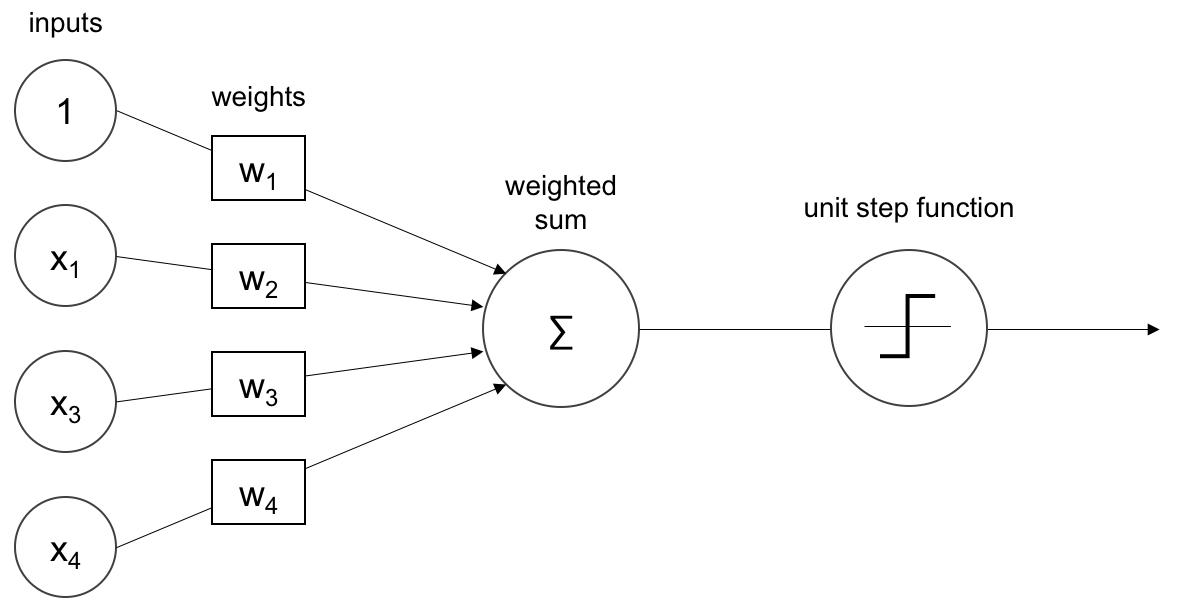
\includegraphics[width=0.6\textwidth]{image3.png}
\caption{The perceptron}
\label{fig:pic3}
\end{figure}

 The weighted sum is passed through a non-linear function called \textit{activation function} to capture the non-linearities in the input.  An \textit{activation function} decides whether a neuron should fire or not. There are various activation functions as shown in \ref{fig:act}. Sigmoid is useful for converting any value to probabilities and can be used for binary classification. The tanh maps input to a value in the range of -1 to 1 and are more stable than sigmoid. The ReLU maps input x to max (0, x) and works well for a large range of problems.
 
\begin{figure}[h]
    \subfigure[Sigmoid function]{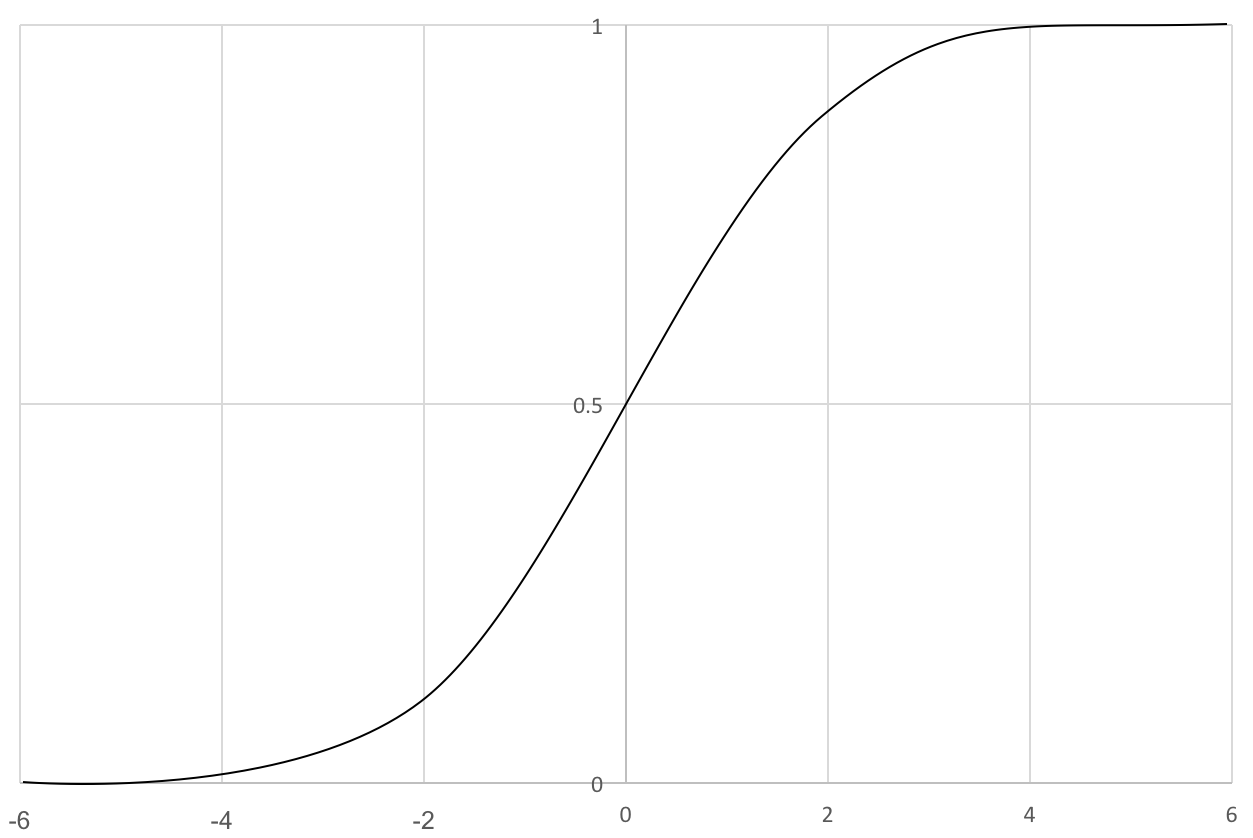
\includegraphics[width=0.30\textwidth]{image4} \label{fig:pic4}}
    \subfigure[Tanh function]{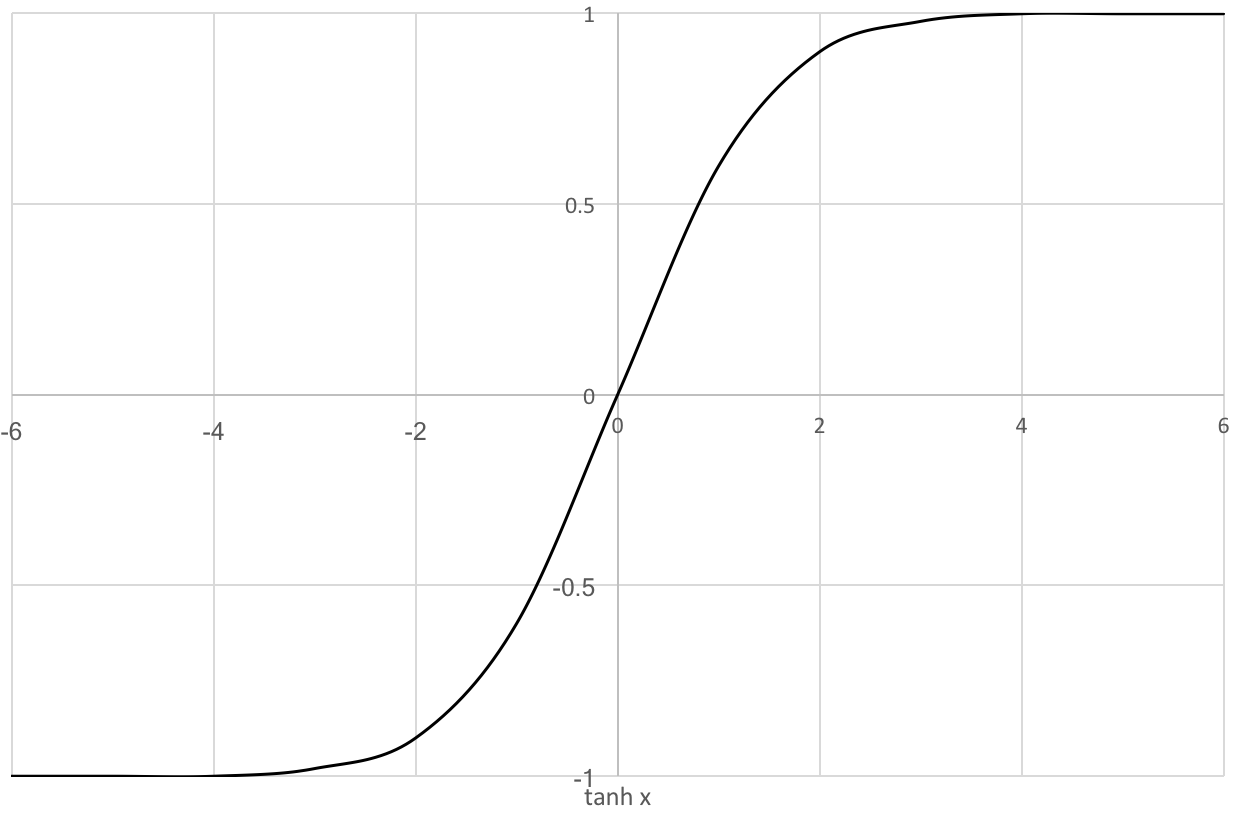
\includegraphics[width=0.30\textwidth]{image5}\label{fig:pic5}}
    \subfigure[RELU function]{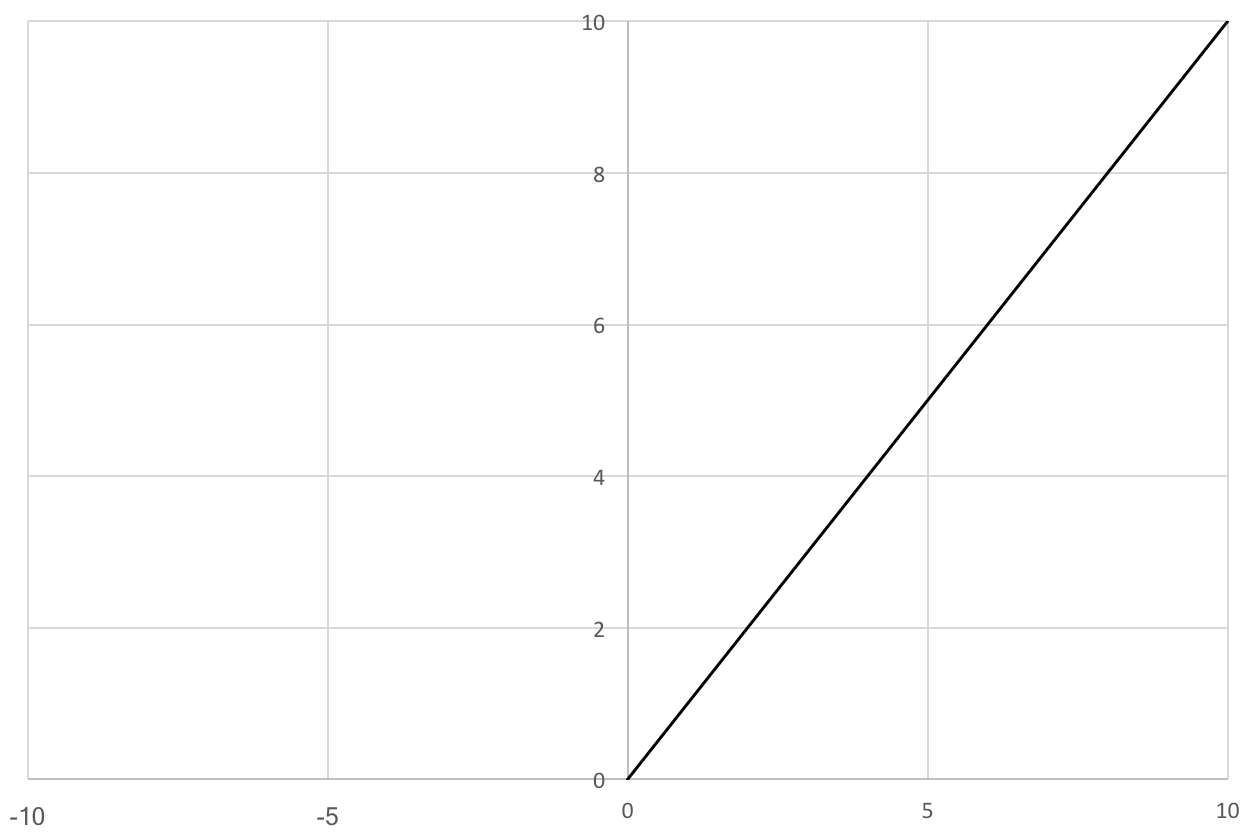
\includegraphics[width=0.30\textwidth]{image6}\label{fig:pic6}}
\caption{Some common activation functions}
\label{fig:act}
\end{figure}


 

\section{Artificial Neural Networks}

Artificial neural network is a collection of perceptrons and activation functions. The perceptrons are connected to each other to form the hidden layers as shown in \ref{fig:pic7}. The training process determines the values of these weights and biases. The training is started by initialising the weights and biases to random values. The error is computed by taking the difference of the actual output to the ground truth. Based on the loss, the weights and biases are tuned in steps. The training is stopped when the error can be minimised anymore and during this point the model is said to learn the features in the input.


\begin{figure}[h]
\centering
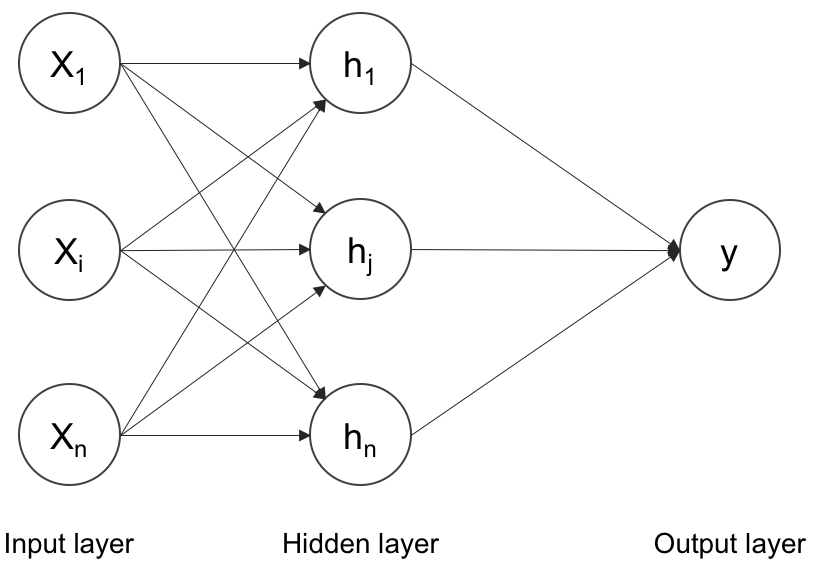
\includegraphics[width=0.6\textwidth]{image7.png}
\caption{Artificial Neural Network}
\label{fig:pic7}
\end{figure}


\section{Training the neural network}

\subsection{Backpropagation}

One of the commonly used algorithm for training the neural networks is the backpropagation algorithm. The weights are updated from the back based on the error that is calculated. The weights are updated using the gradient descent algorithm which is explained in the following section.

\subsection{Gradient Descent}

Often in machine learning, finding the best model for a certain situation means to minimise the error of the model or maximise the likelihood of the data. Hence it can be seen as finding the solution for an optimisation problem. Gradient descent is one of the optimisation problems which is widely used in the algorithms of machine learning and deep learning. 

\subsubsection{Idea}

Suppose we have some function \textbf{f(x)} that takes as input a vector of real numbers and outputs a single real number. One such simple function is given in equation \ref{gradient}. 

\begin{equation} \label{gradient}
f(x) = x^2  \in R
\end{equation}

The \textit{gradient} of \textbf{f(x)} gives the input direction in which the function \textbf{f(x)} most quickly increases. One approach to maximising a function is to pick a random starting point, compute the gradient, take a small step in the direction of the gradient, and repeat with the new starting point. Similarly, we can try to minimise a function by taking small steps in the opposite direction, as shown in \ref{fig:pic0}. 

\begin{figure}[h]
\centering
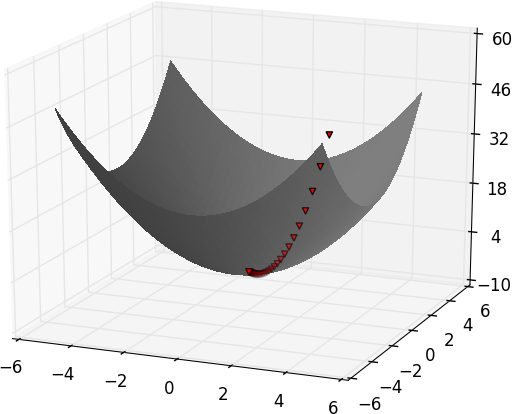
\includegraphics[width=0.6\textwidth]{image1.png}
\caption{Finding a minimum using gradient descent}
\label{fig:pic0}
\end{figure}

This procedure will work very well if the function has a unique global minimum. If a function has multiple (local) minima, this procedure might find the wrong one of them, in which case we might re-run the procedure from a variety of starting points. If a function has no minimum, then it is possible the procedure might go on forever.

\subsubsection{Estimating the gradient}


If f is a function of one variable, its derivative at a point x measures how f(x) changes when we make a very small change to x. The derivative is the slope of the tangent line at (x, f(x)). The gradient can be estimated as given in \ref{eqn:2} by considering h to be very small.

\begin{equation} \label{eqn:2}
Gradient = \frac{f(x+h) - f(x)}{h}
\end{equation}

If f is a function of multiple variables then it has multiple partial derivatives each indicating the change in f when we make small changes to one of the input variables by holding the other variables constant. The learning rate $\eta$ determines the size of the steps we take to reach a (local) minimum. There are three variants of gradient descent as explained in the following sections.

\section{Types of gradient descents }

\subsection{Batch gradient descent}

Batch gradient descent or vanilla gradient descent calculates the gradient of the cost function w.r.t the parameters $\theta$ for the entire training dataset. 

\begin{equation} \label{eqn:3}
\theta = \theta - \eta \cdot \Delta_{\theta} J(\theta)
\end{equation}

Batch gradient descent is slow since we need to calculate the gradients for the whole dataset to make just one update of the parameters. Batch gradient descent is guaranteed to converge to the global minimum for convex error surfaces and to a local minimum for non-convex surfaces.

\subsection{Stochastic gradient descent}

Stochastic gradient descent (SGD) performs parameter update for each training sample. Batch gradient descent performs redundant computations for large gradients since it recomputes the gradients for similar examples before each update. SGD does not have this problem since it performs one update for each training data and is much faster. These frequent updates cause the objective function to fluctuate which may lead to overshooting. However, by setting the optimal learning rate, SGD can show same behaviour as the batch gradient descent.

\begin{equation} \label{eqn:4}
\theta = \theta - \eta \cdot \Delta_{\theta} J(\theta; x^{(i)}; y^{(i)})
\end{equation}


\subsection{Mini-batch gradient descent}

Mini-batch gradient descent takes the best of SGD and batch gradient descent. It updates the parameters for every mini-batch of \textit{n} training samples. It reduces the variance of the parameter updates and hence more stable convergence. It also makes computations more efficient. 

\begin{equation} \label{eqn:5}
\theta = \theta - \eta \cdot \Delta_{\theta} J(\theta; x^{(i:i+n)}; y^{(i:i+n)})
\end{equation}


\subsubsection{Challenges of mini-batch gradient descent}

\begin{itemize}
	\item Finding the optimum learning rate is difficult. A learning rate which is too small will take lots of time to converge and a learning rate too fast might overshoot and oscillate around the minimum.
	\item Neural networks usually have highly non-convex error functions with saddle points. These are the points where one dimension slopes up and another slopes down. The SGD finds these points very hard to escape since the gradient is close to zero in all dimensions.
\end{itemize}

\section{Convolutional Neural Networks}

Convolutional neural networks are very similar to the perceptron. They are made up of neurons with weights and biases. Each neuron performs a product of the input with the weights and adds a non-linearity at the end. They have loss functions and a fully connected layers at the end. However, in convolutional neural networks the inputs are exclusively images which makes the forward propagation easier to implement and also reduces the number of parameters in the network.


\begin{figure}[h]
\centering
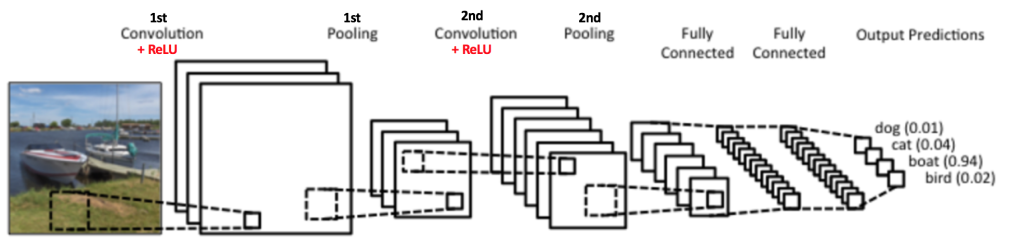
\includegraphics[width=1\textwidth]{image8.png}
\caption{Convolutional layers}
\label{fig:pic8}
\end{figure}
%https://ujjwalkarn.me/2016/08/11/intuitive-explanation-convnets/


The regular neural networks do not scale to full images since they have fully connected layers at the input. For example, an image of 240*480*3 would lead to neurons that have 240*480*3 weights. This would lead to a huge number of parameters and hence to overfitting. In a convolutional neural network, the neurons in a layer will only be connected to a small region of the layer before it, instead of a fully connected network. A convNet is made up of layers and each layer transforms an input 3D volume to an output 3D volume with some differentiable function. The convolution and pooling layers act as feature extractors from the input image and the fully connected layer acts as a classifier. As shown in \ref{fig:pic8} the target probability is 1 for Boat class and 0 for other classes.


\chapter{Transfer learning}

Deep learning networks are \textit{data dependent}. The scale of the model and the size of the data is linearly dependent. Many domains face the problem of insufficient training data. Often the model faces situations where it has not seen the data before and deos not know how to deal with it. In all of such situations the current state-of-the-art models either show degraded performance or even break down. Transfer learning can help us deal with such scenarios.

Tranfer learning allows us to use the already existing labeled data of some related task or domain. The name transfer learning is derived from the fact that we try to transfer as much knowledge as we can from the source to our target task or domain. 

\section{Definition}

Transfer learning involves a domain and a task. A domain \textbf{D} consists of a feature space \textbf{X} and a marginal probability distribution \textbf{P(X)} over the feature space. Given a domain, \textbf{D = (X, P(X))}, a task \textbf{T} consists of a label space \textbf{Y} and a conditional probability distribution \textbf{P(Y$\vert$X)} that is learnt from the training data. Given a source domain \textbf{Ds} and a corresponding source task \textbf{Ts} as well as a target domain \textbf{Dt} and a target task \textbf{Tt}, the objective of transfer learning is to enable to learn the target probability distribution \textbf{P(Yt$\vert$Xt)} in \textbf{Dt} with the information gained from \textbf{Ds} and \textbf{Ts} where  \textbf{Ds} $\neq$ \textbf{Ts} or \textbf{Ts} $\neq$ \textbf{Tt}. 

Given source and target domains \textbf{Ds} and \textbf{Dt} where \textbf{D = (X, P(X))} and source and target tasks \textbf{ts} and \textbf{Tt} where \textbf{T = (Y, P(Y$\vert$X))} there can be four transfer learning scenarios.

\begin{enumerate}
	\item \textbf{Xs} $\neq$ \textbf{Xt}. The feature space of source and target domain are different. 
	\item \textbf{P(Xs)} $\neq$ \textbf{P(Xt)}. Marginal probability distributions of source and target domain are different.
	\item \textbf{Ys} $\neq$ \textbf{Yt}. The label spaces between the two tasks are different.
	\item \textbf{P(Ys$\vert$Xs)} $\neq$ \textbf{P(Yt$\vert$Xt)}. The  conditional probability distributions of the source and target tasks are different.
\end{enumerate}
%Pan, S. J., & Yang, Q. (2010). A survey on transfer learning. IEEE Transactions on Knowledge and Data Engineering, 22(10), 1345–1359.

\section{Transfer learning methods}

Transfer learning has been investigated in the past \cite{noauthor_survey_nodate}. With the approach of deep learning there are new methods of transfer learning available.

\subsection{Using pre-trained CNN features}

%Razavian, A. S., Azizpour, H., Sullivan, J., & Carlsson, S. (2014). CNN features off-the-shelf: An astounding baseline for recognition. IEEE Computer Society Conference on Computer Vision and Pattern Recognition Workshops, 512–519.

This is the most common way of applying transfer learning for a given problem. It is also the method which has been used in this project. The lower layers of the convolutional neural networks capture the low-level image features such as edges, corners etc., while the higher convolutional layers capture more and more complex details such as body parts, faces etc. The final fully connected layers are assumed to capture information that is relevant to solving the respective task for example the classes in case of classification task.
Thus we can simply use the features of a state-of-the-art CNN pre-trained on ImageNet \cite{krizhevsky_imagenet_2012} and train a new model on these extracted features. In practice, we keep the earlier layers of the CNN fixed or tune them with very low learning rate so as to not unlearn these features. This simple approach has been shown to achieve great results on various computer vision tasks \cite{noauthor_survey_nodate}.. Therefore, the ImageNet task seems to be a good base for general computer vision problems. 

\subsection{By developing a model}

In this method, a related predictive modelling problem with an abundance of data is selected and a model is developed based on this task. Then the model is either tuned or reused as is to a different task of interest. 

\chapter{Method}

The aim of the project is to classify the images into three categories based on the head orientation. For this task, the DrivFace dataset \cite{noauthor_uci_nodate} is used which contains images of drivers while driving in real scenarios. We will first consider the data preprocessing, the model, the training and then the testing of the model.

\begin{figure}[h]
    \subfigure[Original image]{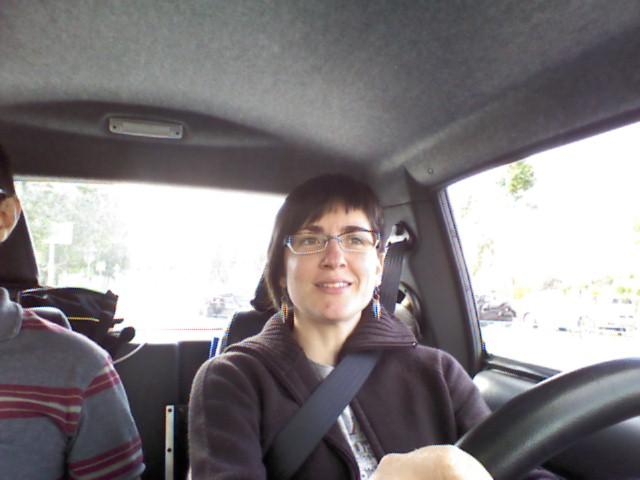
\includegraphics[width=0.49\textwidth]{image10.jpg} \label{fig:pic1}}
    \subfigure[Augumented image]{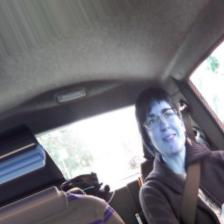
\includegraphics[width=0.37\textwidth]{image9.jpg}\label{fig:pic7}}
\caption{Image augumentation}
\end{figure}

\section{DrivFace Dataset}

The DrivFace database /cite{} contains images sequences of subjects while driving in real scenarios. It is composed of 606 samples of 640—480 pixels each, acquired over different days from 4 drivers (2 women and 2 men) with several facial features like glasses and beard. The ground truth contains the annotation of the face bounding box and the facial key points (eyes, nose and mouth). A set of labels assigning each image into 3 possible gaze direction classes are given.

\begin{enumerate}
	\item The first class is the looking-right class and contains the head angles between -45\degree and -30\degree.
	\item The second one is the frontal class and contains the head angles between -15\degree and 15\degree.
	\item The last one is the looking-left class and contains the head angles between 30\degree and 45\degree.
\end{enumerate}

%\begin{figure}[h]
%    \subfigure[]{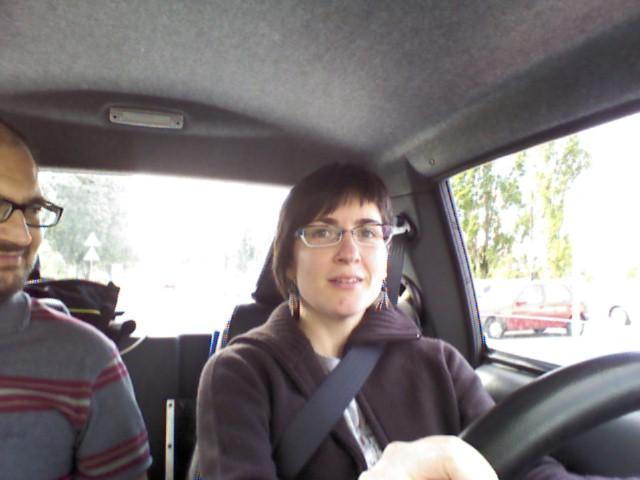
\includegraphics[width=0.37\textwidth]{f.jpg} \label{fig:pic1}}
%    \subfigure[Augumented image]{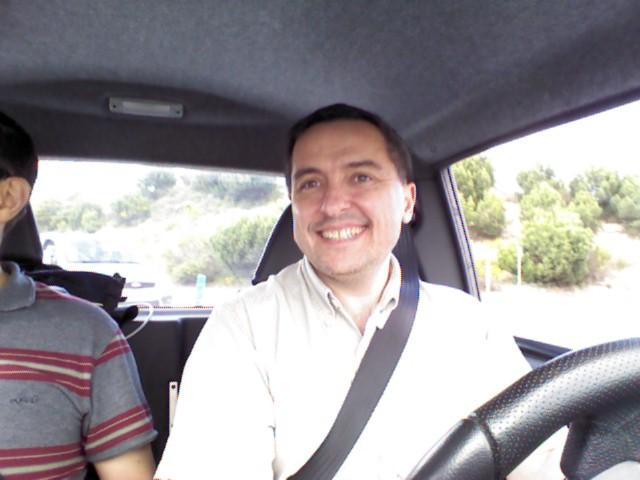
\includegraphics[width=0.37\textwidth]{lr.jpg}\label{fig:pic7}}
%    \subfigure[Augumented image]{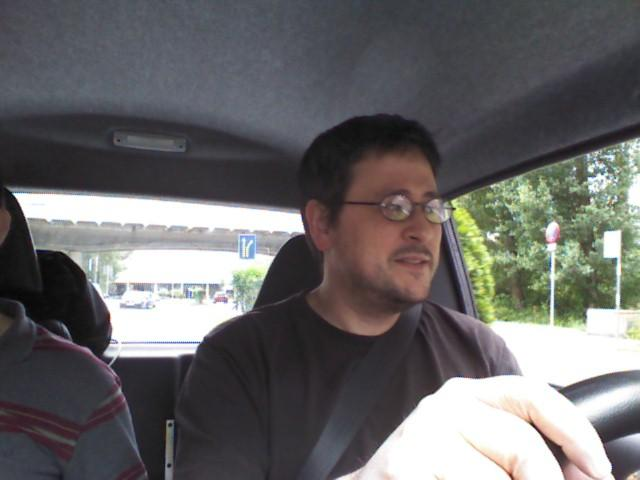
\includegraphics[width=0.37\textwidth]{ll.jpg}\label{fig:pic7}}
%\caption{Image augumentation}
%\end{figure}
 



\section{Preprocess the data}

The data is first augumented using the keras class /textit{ImageDataGenerator}. The parameters of data augumentation are passed while creating an object of the class. Here we set the horizontal flip to false since we need to classify the images as looking left and looking right. We give some rotation ranges, width shift range, height shift range, shear range and zoom range. This generates different augumentated images of our dataset. The images before and after the data augumentation can be seen as below \ref{fig:pic7}. Since the data set already contains the coordinates of the face annotations we use this to extract face from the images. We then split the dataset into train and test with a test data of 20%. 





\section{Model}

We have tested the dataset on four models

\begin{enumerate}
	\item DeepGaze CNN model : The model is derived from the DeepGaze model \cite{noauthor_head_nodate}. There are 9 layers and 4,566,147 parameters as shown in \ref{fig:pic8} 
	\item DeepGaze CNN model with data augumentation: The model is same as the first one but the data is augumented before training. 
	\item Transfer learning with VGGNet: The model uses the first layers as the standard VGGNet model \cite{}. The last layer is removed and replaced with a dense network with 3 neurons each for the 3 outputs.
	\item Transfer learning with ResNet: The model uses the first layers as the standard ResNet50 model \cite{}. The last layer is removed and replaced with a dense network same as the third model.
\end{enumerate}

\begin{figure}[h]
\centering
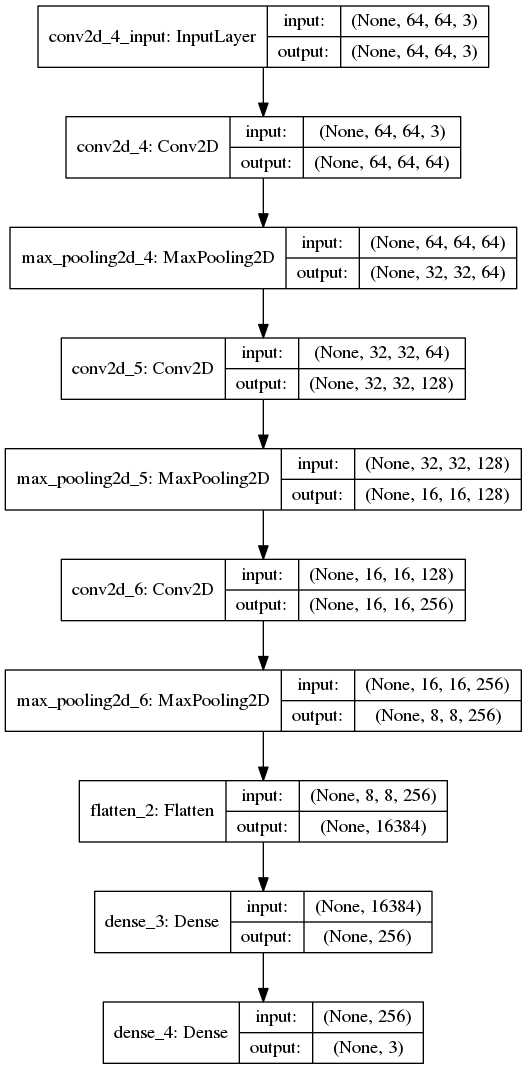
\includegraphics[width=0.33\textwidth]{model_plot_DeepGaze.png}
\caption{DeepGaze CNN Model}
\label{fig:pic8}
\end{figure}

\begin{figure}[h]
\centering
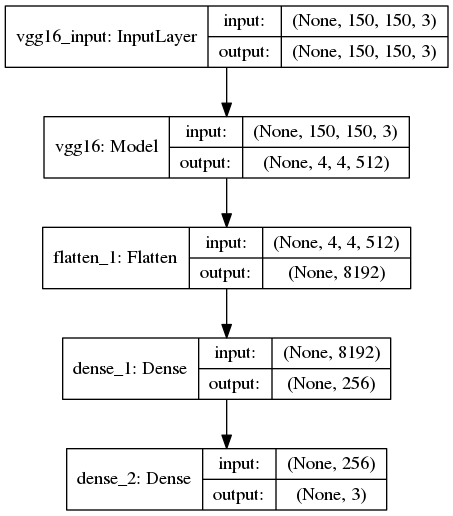
\includegraphics[width=0.5\textwidth]{model_plot_VGG.png}
\caption{VGGNet Model}
\label{fig:pic14}
\end{figure}

\begin{figure}[h]
\centering
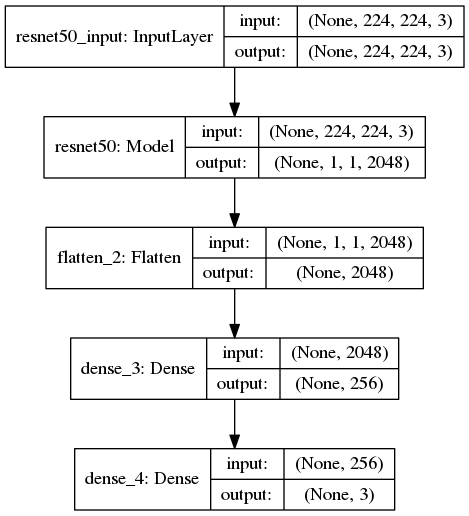
\includegraphics[width=0.5\textwidth]{model_plot_Resnet.png}
\caption{ResNet Model}
\label{fig:pic15}
\end{figure}

\section{Results}

\subsection{DeepGaze Model}

The training and validation accuracy results of the DeepGaze model against the DrivFace dataset is as shown in the figure \ref{fig:pic10}. We can see clearly that the model is overfitting the data since the dataset is too small. Hence the training accuracy soon reaches 100 percent while the validation accuracy keeps dropping. This can be resolved by increasing the size of the dataset using data augumentation. We have used the ImageDataGenerator of Keras \cite{noauthor_keras_nodate} to augument the images before passing them to training. This is done by adding some rotation, translation, shearing, zoom to the images. The horizontal flip is set to false since this modifies the head orientation information in the image. Also, to avoid overfitting dropout regularisation \cite{srivastava_dropout:_2014} technique is added. The results of the training and validation are as shown in the figure \ref{fig:pic11}. The validation accuracy is 84\% with data augumentation which was 62\% without augumentation.


\begin{figure}[h]
    \subfigure[DeepGaze Model without data augumentation]{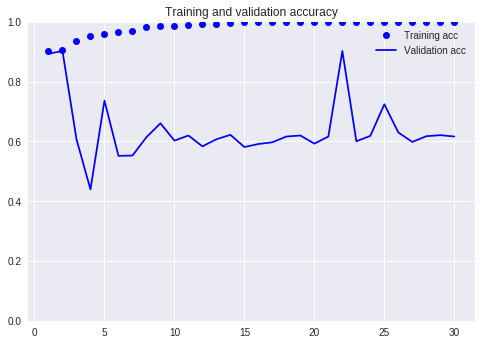
\includegraphics[width=0.5\textwidth]{DeepGaze_No_Aug_Results.png} \label{fig:pic10}}
    \subfigure[DeepGaze Model with data augumentation]{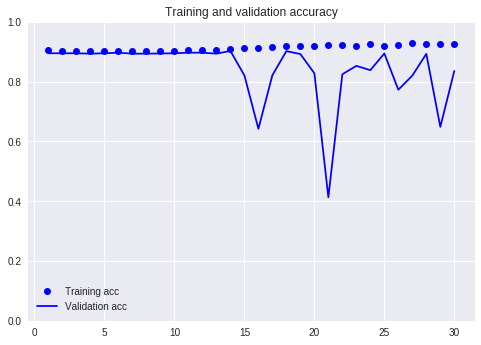
\includegraphics[width=0.5\textwidth]{DeepGaze_Aug_results.png}\label{fig:pic11}}
    \subfigure[VGG16 Model]{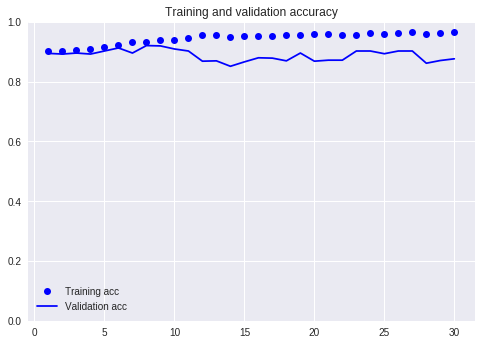
\includegraphics[width=0.5\textwidth]{VGGNet_results.png}\label{fig:pic12}}
    \subfigure[ResNet50]{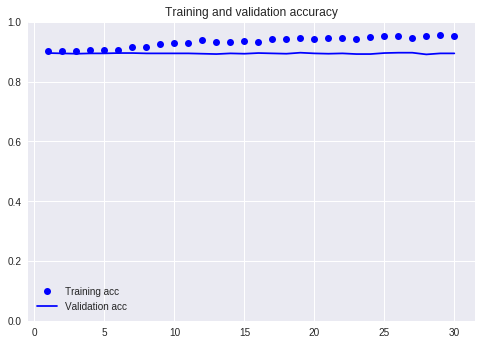
\includegraphics[width=0.5\textwidth]{ResNet_Results.png}\label{fig:pic13}}
\caption{Training vs validation accuracy of the four models}
\end{figure}

\subsection{VGGNet and ResNet Model - Transfer learning}

The training and validation accuracy results of the VGGNet\cite{simonyan_very_2014} and ResNet \cite{noauthor_[1512.03385]_nodate}models are as shown in the figure \ref{fig:pic12} and figure \ref{fig:pic13}. Here, we can see that the problem of overfitting is solved. With the method of transfer learning using VGGNet model, the training and validation curves closely follow each other. But the performance is better with the Resnet model as seen in the figure \ref{fig:pic13}. Also the validation accuracy is 87\% with VGGNet and 89\% with ResNet model. Thus the accuracy problem of the model with less training data is solved by using transfer learning. 



\chapter{Concluding Remarks}
%% Example of, how to use figures

\blindtext

\begin{figure}[h]
\centering

\includegraphics[width=0.6\textwidth]{TU_Chemnitz_positiv_gruen.pdf}
\caption{Graphic 1}
\label{fig:pic0}
\end{figure}

\blindtext
\blindtext

\begin{figure}[h]
    \subfigure[This is the first graphic]{
\includegraphics[width=0.49\textwidth]{TU_Chemnitz_positiv_gruen.pdf} \label{fig:pic1}}
    \subfigure[This is the secound graphic]{
\includegraphics[width=0.49\textwidth]{TU_Chemnitz_positiv_gruen.pdf}\label{fig:pic2}}
\caption{This is the caption of the whole graphic}
\end{figure}

\blindtext

 % Load Data from File example_figures

Head pose estimation is a crucial task in autonomous vehicles since alerting the driver at correct time can prevent several road accidents. It will also help autonomous vehicles to determine the handoff time to the human driver. In this project, various works of head pose estimation were studied. There has been a lot of progress made in head pose estimation systems but not towards systems which can generalize to different drivers, cars, perspective and scale. This model can be further improved by adding several driver gaze zones rather than just three. It was shown that using small datasets causes overfitting and also poor performance. This can be solved by using the approach of transfer learning. We demonstrated that using the state of the art models such as ResNet50, we can solve the overfitting problem and can also achieve significant accuracy. Future work in this direction can use utilize Long Short Term Memory(LSTM) \cite{noauthor_long_nodate} which can use information in successive frames. 

%---------------------------------------------------------
% bibliography based on Springer Design
%---------------------------------------------------------

\bibliographystyle{splncs03}
\bibliography{/Users/adarshmallandur/Desktop/bibliography}

\printindex

\end{document}
